\documentclass[12pt, twoside]{article}
\usepackage[francais]{babel}
\usepackage[T1]{fontenc}
\usepackage[latin1]{inputenc}
\usepackage[left=7mm, right=7mm, top=7mm, bottom=7mm]{geometry}
\usepackage{float}
\usepackage{graphicx}
\usepackage{array}
\usepackage{multirow}
\usepackage{amsmath,amssymb,mathrsfs}
\usepackage{soul}
\usepackage{textcomp}
\usepackage{eurosym}
 \usepackage{variations}
\usepackage{tabvar}

\pagestyle{empty}

\begin{document}

\begin{flushleft}
NOM PRENOM: \ldots \ldots \ldots \ldots \ldots \ldots \ldots \ldots \ldots
 
\bigskip

\end{flushleft}

\begin{center}
{\fbox{$4^{e}3$ \qquad \qquad \textbf{\Large{Contr�le de cours 1 (sujet 1)}}
\qquad \qquad 13/09/2013}}
\end{center}



\bigskip 


\ul{Exercice 1}: Dire si les tableaux suivants sont des tableaux de
proportionnalit� ou non. Expliquer votre r�ponse.

\enskip

\begin{tabular}{cc}

\begin{minipage}{9cm}

Tableau 1:

\enskip

\begin{tabular}{|c|c|c|}
\hline 

2,4 & 5 & 9,4 \\
\hline 
16,8 & 36,5 & 65,8 \\
\hline 
\end{tabular}



\end{minipage}
&
\begin{minipage}{9cm}

Tableau 2:

\enskip

\begin{tabular}{|c|c|c|}
\hline 

4 & 10 & 24 \\
\hline 
8,4 & 21 & 50,4 \\
\hline 
\end{tabular}



\end{minipage}
\end{tabular}

\bigskip


\ldots \ldots \ldots \ldots \ldots \ldots \ldots \ldots \ldots \ldots \ldots
\ldots \ldots \ldots \ldots \ldots \ldots \ldots \ldots \ldots \ldots \ldots
\ldots \ldots \ldots \ldots \ldots \ldots \ldots \ldots \ldots \ldots \ldots
\ldots \ldots 


\ldots \ldots \ldots \ldots \ldots \ldots \ldots \ldots \ldots \ldots \ldots
\ldots \ldots \ldots \ldots \ldots \ldots \ldots \ldots \ldots \ldots \ldots
\ldots \ldots \ldots \ldots \ldots \ldots \ldots \ldots \ldots \ldots \ldots
\ldots \ldots 


\ldots \ldots \ldots \ldots \ldots \ldots \ldots \ldots \ldots \ldots \ldots
\ldots \ldots \ldots \ldots \ldots \ldots \ldots \ldots \ldots \ldots \ldots
\ldots \ldots \ldots \ldots \ldots \ldots \ldots \ldots \ldots \ldots \ldots
\ldots \ldots 

\bigskip

\bigskip

\bigskip


\ul{Exercice 2}: Compl�ter le tableau de proportionnalit� en utilisant la
m�thode la plus appropri�e (�crire les calculs ou mettre des fl�ches dans le
tableau):

\bigskip

\begin{tabular}{cc}
\begin{minipage}{8cm}
\begin{tabular}{|c|c|c|c|c|}
\hline 

2,5 & 5 & 7,5 & \ldots \ldots  & \ldots \ldots \\
\hline 
36 & \ldots \ldots & \ldots \ldots & 18 & 54 \\
\hline 
\end{tabular}
\end{minipage} 
&
\begin{minipage}{10cm}
\ldots \ldots \ldots \ldots \ldots \ldots \ldots \ldots \ldots \ldots \ldots
\ldots \ldots \ldots \ldots \ldots \ldots \ldots 


\ldots \ldots \ldots \ldots \ldots \ldots \ldots \ldots \ldots \ldots \ldots
\ldots \ldots \ldots \ldots \ldots \ldots \ldots 


\ldots \ldots \ldots \ldots \ldots \ldots \ldots \ldots \ldots \ldots \ldots
\ldots \ldots \ldots \ldots \ldots \ldots \ldots 
\end{minipage}

\end{tabular}




\bigskip


\bigskip

\bigskip


\ul{Exercice 3}: Compl�ter les tableaux de proportionnalit� en utilisant la
r�gle des produits en croix (�crivez vos calculs):


\enskip

\begin{tabular}{cc}

\begin{minipage}{9cm}
\begin{tabular}{|c|c|}
\hline 

14 & 63 \\
\hline 
19 & \ldots  \\
\hline 
\end{tabular}





\end{minipage}
&
\begin{minipage}{9cm}

\begin{tabular}{|c|c|}
\hline 

1,8 & \ldots \\
\hline 
2,7 & 39 \\
\hline 
\end{tabular}



\end{minipage}
\end{tabular}


\bigskip

\bigskip

\bigskip


\ul{Exercice 4}: Parmi les graphiques suivants, lesquelles repr�sentent une
situtation de proportionnalit�? Justifier votre r�ponse.

\begin{tabular}{cc}
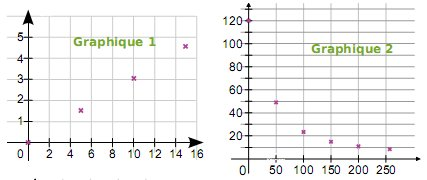
\includegraphics[width=90mm]{images/ex41.jpg} &
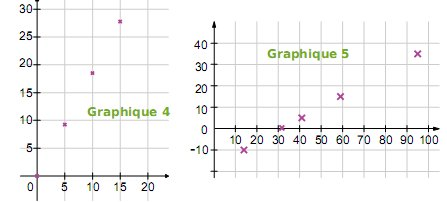
\includegraphics[width=90mm]{images/ex42.jpg} \\
\end{tabular}


\medskip

\ldots \ldots \ldots \ldots \ldots \ldots \ldots \ldots \ldots \ldots \ldots
\ldots \ldots \ldots \ldots \ldots \ldots \ldots \ldots \ldots \ldots \ldots
\ldots \ldots \ldots \ldots \ldots \ldots \ldots \ldots \ldots \ldots \ldots
\ldots \ldots 


\ldots \ldots \ldots \ldots \ldots \ldots \ldots \ldots \ldots \ldots \ldots
\ldots \ldots \ldots \ldots \ldots \ldots \ldots \ldots \ldots \ldots \ldots
\ldots \ldots \ldots \ldots \ldots \ldots \ldots \ldots \ldots \ldots \ldots
\ldots \ldots 


\ldots \ldots \ldots \ldots \ldots \ldots \ldots \ldots \ldots \ldots \ldots
\ldots \ldots \ldots \ldots \ldots \ldots \ldots \ldots \ldots \ldots \ldots
\ldots \ldots \ldots \ldots \ldots \ldots \ldots \ldots \ldots \ldots \ldots
\ldots \ldots 



\pagebreak



\begin{flushleft}
NOM PRENOM: \ldots \ldots \ldots \ldots \ldots \ldots \ldots \ldots \ldots
 
\bigskip

\end{flushleft}

\begin{center}
{\fbox{$4^{e}3$ \qquad \qquad \textbf{\Large{Contr�le de cours 1 (sujet 2)}}
\qquad \qquad 13/09/2013}}
\end{center}

  

\bigskip 


\ul{Exercice 1}: Dire si les tableaux suivants sont des tableaux de
proportionnalit� ou non. Expliquer votre r�ponse.

\enskip

\begin{tabular}{cc}

\begin{minipage}{9cm}

Tableau 1:

\enskip

\begin{tabular}{|c|c|c|}
\hline 

 6 & 4 & 11 \\
\hline 
14,4 & 9,6 & 26,4 \\
\hline 
\end{tabular}



\end{minipage}
&
\begin{minipage}{9cm}

Tableau 2:

\enskip

\begin{tabular}{|c|c|c|}
\hline 

2,6 & 7 & 10,1 \\
\hline 
18,2 & 42 & 60,6 \\
\hline 
\end{tabular}



\end{minipage}
\end{tabular}

\bigskip


\ldots \ldots \ldots \ldots \ldots \ldots \ldots \ldots \ldots \ldots \ldots
\ldots \ldots \ldots \ldots \ldots \ldots \ldots \ldots \ldots \ldots \ldots
\ldots \ldots \ldots \ldots \ldots \ldots \ldots \ldots \ldots \ldots \ldots
\ldots \ldots 


\ldots \ldots \ldots \ldots \ldots \ldots \ldots \ldots \ldots \ldots \ldots
\ldots \ldots \ldots \ldots \ldots \ldots \ldots \ldots \ldots \ldots \ldots
\ldots \ldots \ldots \ldots \ldots \ldots \ldots \ldots \ldots \ldots \ldots
\ldots \ldots 


\ldots \ldots \ldots \ldots \ldots \ldots \ldots \ldots \ldots \ldots \ldots
\ldots \ldots \ldots \ldots \ldots \ldots \ldots \ldots \ldots \ldots \ldots
\ldots \ldots \ldots \ldots \ldots \ldots \ldots \ldots \ldots \ldots \ldots
\ldots \ldots 

\bigskip

\bigskip

\bigskip


\ul{Exercice 2}: Compl�ter le tableau de proportionnalit� en utilisant la
m�thode la plus appropri�e (�crire les calculs ou mettre des fl�ches dans le
tableau):

\bigskip

\begin{tabular}{cc}
\begin{minipage}{8cm}
\begin{tabular}{|c|c|c|c|c|}
\hline 

1,5 &  3 & 4,5 & \ldots \ldots  & \ldots \ldots \\
\hline 
28 & \ldots \ldots & \ldots \ldots & 14 & 42 \\
\hline 
\end{tabular}
\end{minipage} 
&
\begin{minipage}{10cm}
\ldots \ldots \ldots \ldots \ldots \ldots \ldots \ldots \ldots \ldots \ldots
\ldots \ldots \ldots \ldots \ldots \ldots \ldots 


\ldots \ldots \ldots \ldots \ldots \ldots \ldots \ldots \ldots \ldots \ldots
\ldots \ldots \ldots \ldots \ldots \ldots \ldots 


\ldots \ldots \ldots \ldots \ldots \ldots \ldots \ldots \ldots \ldots \ldots
\ldots \ldots \ldots \ldots \ldots \ldots \ldots 
\end{minipage}

\end{tabular}




\bigskip


\bigskip

\bigskip


\ul{Exercice 3}: Compl�ter les tableaux de proportionnalit� en utilisant la
r�gle des produits en croix (�crivez vos calculs):


\enskip

\begin{tabular}{cc}

\begin{minipage}{9cm}
\begin{tabular}{|c|c|}
\hline 

17 & 85 \\
\hline 
21 & \ldots  \\
\hline 
\end{tabular}





\end{minipage}
&
\begin{minipage}{9cm}

\begin{tabular}{|c|c|}
\hline 

1,6 & \ldots \\
\hline 
2,8 & 21 \\
\hline 
\end{tabular}



\end{minipage}
\end{tabular}


\bigskip

\bigskip

\bigskip


\ul{Exercice 4}: Parmi les graphiques suivants, lesquelles repr�sentent une
situtation de proportionnalit�? Justifier votre r�ponse.

\enskip


\begin{center}
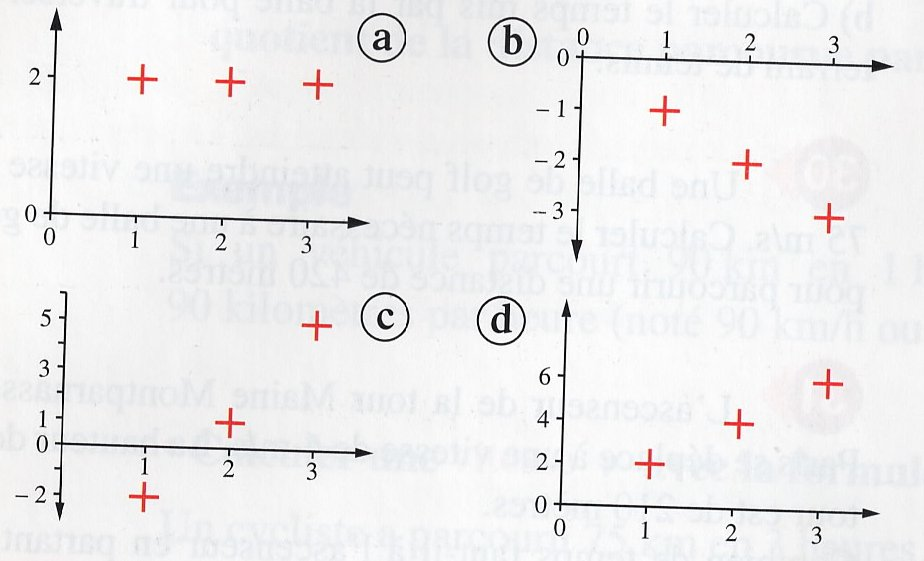
\includegraphics[width=10cm]{images/ex43.jpg}
\end{center}

\medskip

\ldots \ldots \ldots \ldots \ldots \ldots \ldots \ldots \ldots \ldots \ldots
\ldots \ldots \ldots \ldots \ldots \ldots \ldots \ldots \ldots \ldots \ldots
\ldots \ldots \ldots \ldots \ldots \ldots \ldots \ldots \ldots \ldots \ldots
\ldots \ldots 


\ldots \ldots \ldots \ldots \ldots \ldots \ldots \ldots \ldots \ldots \ldots
\ldots \ldots \ldots \ldots \ldots \ldots \ldots \ldots \ldots \ldots \ldots
\ldots \ldots \ldots \ldots \ldots \ldots \ldots \ldots \ldots \ldots \ldots
\ldots \ldots 


\ldots \ldots \ldots \ldots \ldots \ldots \ldots \ldots \ldots \ldots \ldots
\ldots \ldots \ldots \ldots \ldots \ldots \ldots \ldots \ldots \ldots \ldots
\ldots \ldots \ldots \ldots \ldots \ldots \ldots \ldots \ldots \ldots \ldots
\ldots \ldots
\end{document}
